\newpage
\section{Rendering Process}
\label{sec:rendering_process}
\hspace{\parindent}
looking at the render process of any graphics engine can give one a valuable lesson, as the exact details may differ depending on used technology and implementation. This section is a step by step presentation of the rendering process in TSEngine.\\
\begin{figure}[H]
  \includegraphics[width=\linewidth]{frame_generation/part1-3.png}
  \caption{Rendering process steps 1-3}
\end{figure}
In the first step, one can see an empty frame. It, as well as all others shown in this section, are consecutive framebuffers stored in GPU memory.
Secondly, the predefined grid is rendered, creation of which was inspired by the series of articles \textit{"Borderland between Rendering and Editor"} \cite{GridRendering}.
In the next steps, TSEngine loads all entities. Order of rendering them is dependent on each entity's \texttt{z value}. In this provided example environment, the first rendered entity is the village, which mesh component is the village model \cite{VillageModel}.

\begin{figure}[H]
  \includegraphics[width=\linewidth]{frame_generation/part4-6.png}
  \caption{Rendering process steps 4-6}
\end{figure}
% TODO: we should include polonez.obj in refs
The fourth step is similar to the previous one, it only renders polonez entity with \texttt{polonez.obj} \cite{PolonezModel} file as its mesh component. It could be useful to mention that both village and polonez entities are rendered with normal lightning and don't use physically based shading.
Conversely, in the fifth step, the sphere entity that is rendered, takes full advantage of physically based rendering implemented in the TSEngine. In its renderer component, it uses PBR with gold as material. 
The sixth step is almost the same as the last one - it renders a sphere. The only difference is a slight offset in comparison to the sphere rendered in the fifth step.

\begin{figure}[H]
  \includegraphics[width=\linewidth]{figures/frame_generation/part7-9.png}
  \caption{Rendering process steps 7-9}
\end{figure}
The seventh step is the last one rendering a sphere, again, the sphere is the exact replica of its predecessors, excluding the offset. The three sphere entities were implemented via a simple loop and are the same, save for their tags and positions.
In the eight step, finally some change can be observed - the frame has a source of light now. It is also an entity with renderer component with template variable, specifying that this is a light.
The frame in the ninth step is visually the same as the eight frame. It is because in this step the second light, that is off-screen, is rendered.
\begin{figure}[H]
  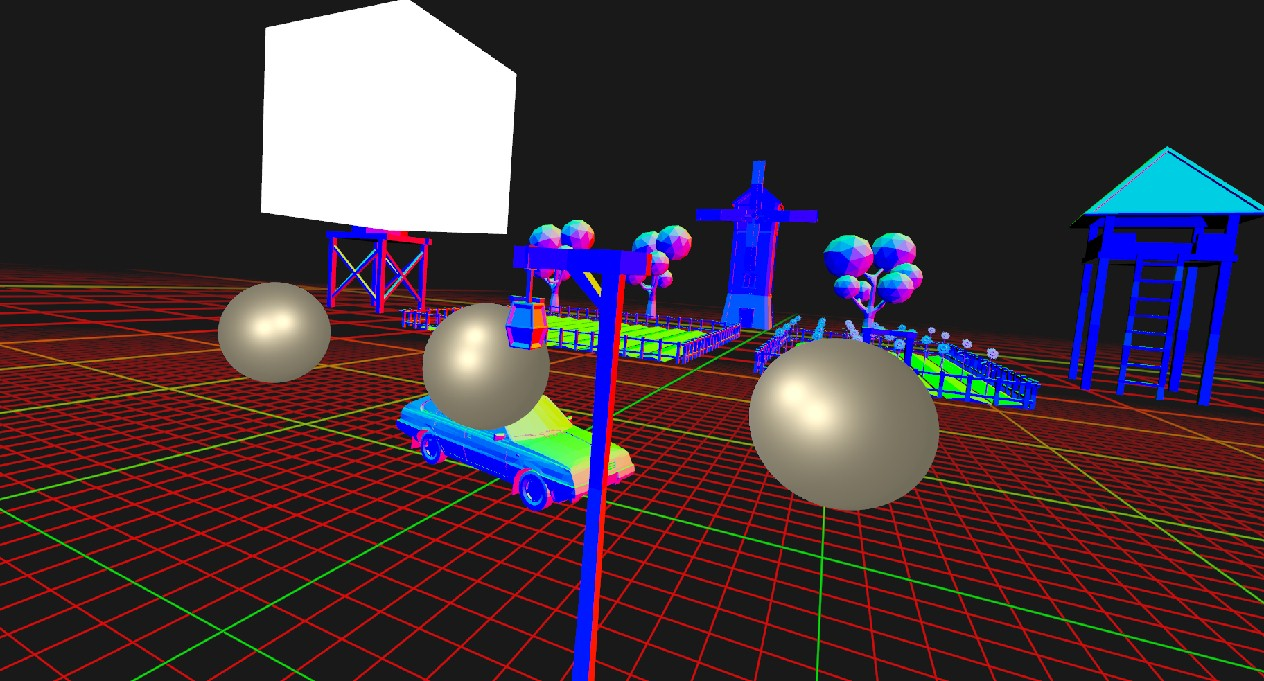
\includegraphics[width=\linewidth]{frame_generation/part10.jpg}
  \caption{Rendering process step 10}
\end{figure}
The tenth and final frame as one can see has different proportions compared to the previous frames. It is so, because all the previous frames were framebuffers of the headset and this one is a framebuffer of the mirrored window displayed on the monitor.
